\chapter{The Lie Algebra of Markov Process Generators}
In which we develop and explore the containing Lie algebras of the generators of continuous
time homogeneous Markov processes on finite-state spaces.
\section{Stochastic Matrices}
\subsection{Preliminaries}
The classical Lie algebras of physics, like the infinitesimal symmetries of the special
unitary algebra $\mathfrak{su}(n)$, are defined with respect to invariants of a Banach
algebra, such as the matrix invariants of the determinant, trace, or norm. In contrast,
stochastic matrices are always characterized with respect to a choice of a specific single
subspace spanned by a vector of unit norm. For reasons that will become clear later, we will
denote this characterizing unit vector by $\hat{\mathbbm{1}}$
\footnote{For the remainder of the text vectors will be denoted with the over arrow $\vec{v}$, and vectors of unit norm will be denoted with the hat $\hat{u}$; so that $\left\| \hat{u} \right\| = 1$}. In the next two sections we 
will provide an explicit construction and characterization of the Lie algebra of stochastic 
matrices, building on the original work of Johnson \cite{johnson_markov-type_1985} and
distilling the recent works of Sumner et al. \cite{sumner_lie_2012,fernandez-sanchez_lie_2012} 
Mourad \cite{mourad_lie-theoretic_2004} and Chruściński et al. \cite{chruscinski_pseudo-stochastic_2015}.

The common approach to stochastic matrices begins with the restriction that a matrix $A$ has 
non-negative entries with respect to the standard orthonormal basis for the vector space on 
which it acts; namely $\left\langle\hat{e}_i,A \hat{e}_j\right\rangle \ge 0$ for all $i,j$. 
In addition to allowing for singular matrices, this poses an immediate obstacle to the 
necessary closure with respect to matrix inversion required for matrix groups; as the 
inverse of a stochastic matrix need not have non-negative entries with respect to the
standard orthonormal basis. 

For the moment we will set aside the restriction that the entries be non-negative, and
instead begin with a generalization of fixed row sums to abstract linear operators. We will
show that this generalization is preserved by operator inversion, and then develop an
orthonormal basis from which matrix representations of the abstract linear operators can be
constructed with non-negative entries. In essence tackling the problem from the reverse
direction, starting with an abstract generalization of the idea of fixed row sums and then 
specifying matrices with non-negative entries with respect to a constructed orthonormal
basis.
\begin{definition}
	A bounded linear operator $A$ on a finite dimensional Hilbert space is stochastic with
	respect to the unit vector $\hat{\mathbbm{1}}$ if $A \hat{\mathbbm{1}} = \hat{\mathbbm{1}}$
\end{definition}
Note that this definition does not stipulate any conditions on non-singularity, and thus
includes, as representations of the linear operators, all the matrices in the convex
polytope of stochastic matrices. For an $n$ dimensional vector space the vector $\vec{\mathbbm{1}} = \sqrt{n} \hat{\mathbbm{1}}$
acts as the row sum operator on bounded linear operators stochastic with respect to $\hat{\mathbbm{1}}$. 
We will make this claim more precise after we dispense with a few more foundational
definitions.
\begin{definition}
	Let $St(\hat{\mathbbm{1}})$ denote the stochastic Lie group of invertible bounded linear
	operators stochastic with respect to $\hat{\mathbbm{1}}$.
\end{definition}
It is tempting to view the name stochastic Lie group as a bait and switch, or at least an
abuse of the terminology, given we have removed the usual convex polytope of stochastic
matrices and replaced it with a group of invertible bounded linear operators with a common
eigenvector $\hat{\mathbbm{1}}$. Previous authors have denoted the convex polytope of
stochastic matrices as the stochastic semi-group, and the group of invertible matrices as
the pseudo-stochastic Lie group. One could even consider incorporating Markov into the name,
in reference to the fact that the transition matrices of a continuous time homogeneous
Markov process on a finite-state space are by definition invertible, and have common
eigenvector $\hat{\mathbbm{1}}$. However the suffix of Lie group in the name connotes both
sufficient additional restrictions to make the name distinct, and still allows for an
indication of a relationship with the original concept. Of course, this definition
immediately necessitates a proof of the claim embedded in the definition.
\begin{lemma}
	$St(\hat{\mathbbm{1}})$ is a Lie group.
\end{lemma}
\begin{IEEEproof}
	We proceed by working mechanistically through the Lie group axioms \cite{hall_lie_2004}.
	\begin{enumerate}
		\item The identity element $I$ is in $St(\hat{\mathbbm{1}})$. Clearly $I$ is invertible
		and $I \hat{\mathbbm{1}} = \hat{\mathbbm{1}}$.
		\item If $A,B \in St(\hat{\mathbbm{1}})$ then $AB \in St(\hat{\mathbbm{1}})$. This
		follows from the computation $AB \hat{\mathbbm{1}} = A \hat{\mathbbm{1}} = \hat{\mathbbm{1}}$.
		\item If $A \in St(\hat{\mathbbm{1}})$ then $A^{-1} \in St(\hat{\mathbbm{1}})$.
		Recognize that $A \hat{\mathbbm{1}} = \hat{\mathbbm{1}}$ implies $\hat{\mathbbm{1}} = A^{-1} A \hat{\mathbbm{1}} = A^{-1} \hat{\mathbbm{1}}$.
		\item Associativity follows from $St(\hat{\mathbbm{1}})$ being a subgroup of $GL\left(n\right)$.
		\item Finally, we need to prove that $St(\hat{\mathbbm{1}})$ is closed within $GL\left(n\right)$.
		Consider a sequence $A_n \in St(\hat{\mathbbm{1}})$ that converges to $A$, then $\hat{\mathbbm{1}} = A_n \hat{\mathbbm{1}} \rightarrow A \hat{\mathbbm{1}}$. 
		Now if $A$ is invertible then we are done, and if $A$ is not invertible then $A \notin GL\left(n\right)$,
		again satisfying closure within $GL\left(n\right)$.\hfill\IEEEQEDhere
	\end{enumerate}
\end{IEEEproof}
That $St(\hat{\mathbbm{1}})$ is a proper Lie group implies that it must be infinitesimal
generated by elements of a Lie algebra.
\begin{definition}
	Let $\mathfrak{st}(\hat{\mathbbm{1}})$ denote the stochastic Lie algebra of $St(\hat{\mathbbm{1}})$.
\end{definition}
By infinitesimally generated we mean that every element of $St(\hat{\mathbbm{1}})$ is the
exponential map of at least one element in $\mathfrak{st}(\hat{\mathbbm{1}})$. We can fully
characterize this algebra as the set of bounded linear operators such that $\hat{\mathbbm{1}}$
is in the kernel of each operator.
\begin{lemma}
	The algebra $\mathfrak{st}(\hat{\mathbbm{1}})$ is exactly the set of all bounded linear
	operators with $\hat{\mathbbm{1}}$ in their kernel.
\end{lemma}
\begin{IEEEproof}
	Working through the forward and backward inclusions we have
	\begin{enumerate}
		\item Suppose $A \hat{\mathbbm{1}} = 0$ then from the definition of the exponential map
		we have:
		\begin{IEEEeqnarray*}{rCl}
			\exp\left(A\right) \hat{\mathbbm{1}}
				& = & \sum_{n=0}^{\infty} \frac{1}{n!} A^n \hat{\mathbbm{1}}\\
				& = & \hat{\mathbbm{1}} + \sum_{n=1}^{\infty} \frac{1}{n!} 0\\
				& = & \hat{\mathbbm{1}}
		\end{IEEEeqnarray*}
		Thus $\exp\left(A\right) \in St(\hat{\mathbbm{1}})$ implying that $A \in \mathfrak{st}(\hat{\mathbbm{1}})$
		\item Now proceeding with the reverse assumption, that $A \in \mathfrak{st}(\hat{\mathbbm{1}})$.
		For all $t \in \mathbb{R}$ we have $\exp\left(tA\right) \hat{\mathbbm{1}} = \hat{\mathbbm{1}}$.
		Differentiating $\hat{\mathbbm{1}}$ with respect to $t$ and evaluating at $t = 0$ yields
		\begin{IEEEeqnarray*}{+rCl+x*}
			0 & = & \left. \frac{d}{dt} \hat{\mathbbm{1}} \right|_{t=0}\\
				& = & \left. \frac{d}{dt} \exp\left(tA\right) \hat{\mathbbm{1}} \right|_{t=0}\\
				& = & \left. \exp\left(tA\right) A \hat{\mathbbm{1}} \right|_{t=0}\\
				& = & A \hat{\mathbbm{1}} & \IEEEQEDhere
		\end{IEEEeqnarray*}
	\end{enumerate}
\end{IEEEproof}
The following chapter will hinge on taking the derivatives of smooth parameterizations $X : \mathbb{R}^k \mapsto \mathfrak{st}(\hat{\mathbbm{1}})$. 
The principle role of this chapter is to assure ourselves that we will not differentiate
ourselves out of $\mathfrak{st}(\hat{\mathbbm{1}})$. The next corollary nicely provides just
such an assurance:
\begin{corollary}
	The tangent space $T\mathfrak{st}(\hat{\mathbbm{1}}) = \mathfrak{st}(\hat{\mathbbm{1}})$.
\end{corollary}
\begin{IEEEproof}
	The proof is complementary to the preceding lemma and moves through each direction of
	inclusion:
	\begin{enumerate}
		\item To show that $\mathfrak{st}(\hat{\mathbbm{1}})\subseteq T\mathfrak{st}(\hat{\mathbbm{1}})$
		consider $X\left(x\right) = x X_0$ where $x$ is a complex scalar parameter and $X_0 \in \mathfrak{st}(\hat{\mathbbm{1}})$.
		\item By construction $X\left(x\right) \in \mathfrak{st}(\hat{\mathbbm{1}})$, because $X_0 \in \mathfrak{st}(\hat{\mathbbm{1}})$
		and $\mathfrak{st}(\hat{\mathbbm{1}})$ is a vector space; so multiplication by the 
		complex scalar parameter $x$ will always reside in $\mathfrak{st}(\hat{\mathbbm{1}})$.
		\item Furthermore the tangent $\frac{\partial}{\partial x} X\left(x\right) = X_0 \in \mathfrak{st}(\hat{\mathbbm{1}})$.
		\item Now to show that $T \mathfrak{st}(\hat{\mathbbm{1}}) \subseteq \mathfrak{st}(\hat{\mathbbm{1}})$
		we start with an arbitrary smooth parameterization $X\left(x\right) : \mathbb{R}^k \mapsto \mathfrak{st}(\hat{\mathbbm{1}})$.
		\item Using the same trick of differentiation we have
		\begin{IEEEeqnarray*}{+rCl+x*}
			0 & = & \frac{\partial}{\partial x} 0\\
				& = & \frac{\partial}{\partial x} \left( X\left(x\right) \hat{\mathbbm{1}}\right)\\
				& = & \left(\frac{\partial}{\partial x} X\left(x\right)\right) \hat{\mathbbm{1}} & \IEEEQEDhere
		\end{IEEEeqnarray*}
	\end{enumerate}
\end{IEEEproof}
Clearly the tangent space to a normed vector space is the normed vector space. After all one
can just choose a fixed basis and then differentiate the individual smoothly parameterized
in projections. However, the proof of the preceding corollary was constructed to explicitly
connect algebraic closure and differentiation, with the norm implicitly used in the
differentiation. The proof further illustrates the intuition that any increase in a
particular matrix element has to be compensated for by an equal decrease in some other
matrix elements.
\subsection{Canonical Generators}
Over an $n$ dimensional vector space, the condition on a matrix $A$ that $A \hat{\mathbbm{1}} = 0$
places $n$ constraints on the $n^2$ dimensions of $A$. This leaves $n^2 - n$ free dimensions
on $\mathfrak{st}(\hat{\mathbbm{1}})$, when considered as a vector space. This hints that we
can construct a generator of $\mathfrak{st}(\hat{\mathbbm{1}})$ from order pairs of basis
elements $\hat{e}_i$ for the vector space of $\hat{\mathbbm{1}}$. To see how this is done we
first construct a useful basis for the vector space to which $\hat{\mathbbm{1}}$ is a
member.
\begin{lemma}
	There exists an orthonormal basis $\hat{e}_i$, indexed by $1 \le i \le n$, such that $\left\langle \hat{e}_i, \hat{\mathbbm{1}} \right\rangle = \frac{1}{\sqrt{n}}$.
\end{lemma}
\begin{IEEEproof}
	While a basis with the stipulated properties can be constructed through the Gram-Schmidt
	process, the proof of the existence proceeds by induction.
	\begin{enumerate}
		\item For $n=1$ the desired basis is precisely the trivial set $\left\lbrace \hat{\mathbbm{1}} \right\rbrace$ 
		which satisfies the condition that $\left\langle \hat{\mathbbm{1}}, \hat{\mathbbm{1}} \right\rangle = 1$.
		\item Assume the claim is true for $n$. For $n+1$ pick a unit vector $\hat{e}_{\perp}$
		that is orthogonal to $\hat{\mathbbm{1}}$ and construct the unit vector
		$\hat{e}_{n+1} = \frac{1}{\sqrt{n+1}} \hat{\mathbbm{1}} + \sqrt{\frac{n}{n+1}} \hat{e}_{\perp}$.
		Clearly $\hat{e}_{n+1}$ satisfies the condition $\left\langle \hat{e}_{n+1}, \hat{\mathbbm{1}} \right\rangle = \frac{1}{\sqrt{n+1}}$.
		\item To use the induction assumption we construct a new row sum unit vector $\hat{\mathbbm{1}}_n = \sqrt{\frac{n+1}{n}}\hat{\mathbbm{1}} - \frac{1}{\sqrt{n}}\hat{e}_{n+1}$ 
		in one dimension lower by projecting onto the subspace orthogonal to $\hat{e}_{n+1}$.
		\item By the induction assumption there exists a basis $\hat{e}_i$ with $i \le n$, such
		that $\left\langle \hat{e}_i, \hat{\mathbbm{1}}_n \right\rangle = \frac{1}{\sqrt{n}}$.
		\item Because $\hat{e}_i$ with $i \le n$ was constructed in the space orthogonal to $\hat{e}_{n+1}$
		it follows that $\left\langle \hat{e}_i, \hat{e}_j \right\rangle = \delta_{ij}$ for all
		$i,j \le n+1 $.
		\item Then using the definitions of $\hat{e}_{n+1}$ and $\hat{\mathbbm{1}}_n$ we can
		calculate the inner product $\left\langle \hat{e}_i, \hat{\mathbbm{1}}_n \right\rangle$
		for $i \le n$
		\begin{IEEEeqnarray*}{rCl}
			\frac{1}{\sqrt{n}}
				& = & \left\langle \hat{e}_i, \hat{\mathbbm{1}}_n \right\rangle\\
				& = & \sqrt{\frac{n+1}{n}} \left\langle \hat{e}_j, \hat{\mathbbm{1}} \right\rangle - \frac{1}{\sqrt{n}} \left\langle \hat{e}_i, \hat{e}_{n+1} \right\rangle\\
				& = & \sqrt{\frac{n+1}{n}} \left\langle \hat{e}_j, \hat{\mathbbm{1}} \right\rangle
		\end{IEEEeqnarray*}
		Inverting the fraction in the equality yields $\left\langle \hat{e}_i, \hat{\mathbbm{1}} \right\rangle = \frac{1}{\sqrt{n+1}}$
		for all $i \le n+1$.\hfill\IEEEQEDhere
	\end{enumerate}
\end{IEEEproof}
As a direct result of the construction of the basis vectors $\hat{e}_i$ we see that $\vec{\mathbbm{1}} = \sum_{i=1}^n \hat{e}_i$.
Thus $\vec{\mathbbm{1}}$ can be interpreted as the row sum vector in basis $\hat{e}_i$.

The constructed basis leads naturally to considering the minimal non-trivial matrices $C_{ij} = \hat{e}_i \otimes \left( \hat{e}_j - \hat{e}_i \right)$,
as holding significance in the structure of $\mathfrak{st}(\hat{\mathbbm{1}})$. These 
matrices are illustrated as state transitions in figure \ref{fig:singlestochastic}. In fact, 
this will be the central result of this chapter: the algebraic closure of the matrices $C_{ij}$
is the stochastic Lie algebra $\mathfrak{st}(\hat{\mathbbm{1}})$. To establish this result 
we need a preliminary result that proves the commutators $\left[C_{ij},C_{kl}\right]$ are 
linear combinations of matrices $C_{ij}$.
\begin{lemma}
	\begin{IEEEeqnarray*}{rCl}
		C_{ij}C_{kl} & = &
		\begin{cases}
			- C_{il} & i=k,\\
			C_{il} - C_{ij} & j=k,\\
			0 & \text{otherwise}.
		\end{cases}
	\end{IEEEeqnarray*}
\end{lemma}
\begin{IEEEproof}
	We proceed in two steps; calculating the terms of the products, then simplifying the 
	cases, always assuming $i \neq j$ and $k \neq l$.
	\begin{enumerate}
		\item Term wise computation of the Kronecker products yields
		\begin{IEEEeqnarray*}{rCl}
			C_{ij}C_{kl}
				& = & \hat{e}_i \otimes \left( \hat{e}_j - \hat{e}_i \right) \hat{e}_k \otimes \left( \hat{e}_l - \hat{e}_k \right)\\
				& = & \hat{e}_i \otimes \hat{e}_j \hat{e}_k \otimes \hat{e}_l + \hat{e}_i \otimes \hat{e}_i \hat{e}_k \otimes \hat{e}_k - \hat{e}_i \otimes \hat{e}_j \hat{e}_k \otimes \hat{e}_k - \hat{e}_i \otimes \hat{e}_i \hat{e}_k \otimes \hat{e}_l\\
				& = & \delta_{jk} \hat{e}_i \otimes \hat{e}_l + \delta_{ik} \hat{e}_i \otimes \hat{e}_k - \delta_{jk} \hat{e}_i \otimes \hat{e}_k - \delta_{ik} \hat{e}_i \otimes \hat{e}_l\\
				& = & \left(\delta_{jk} - \delta_{ik} \right) \hat{e}_i \otimes \left( \hat{e}_l - \hat{e}_k \right)
		\end{IEEEeqnarray*}
		\item We work through each case of $\delta_{jk} - \delta_{ik}$, starting with the case $i=k$ 
		\begin{IEEEeqnarray*}{rCl}
			C_{ij}C_{il}
				& = & \left(\delta_{jk} - \delta_{ii} \right) \hat{e}_i \otimes \left( \hat{e}_l - \hat{e}_i \right)\\
				& = & - \hat{e}_i \otimes \left( \hat{e}_l - \hat{e}_i \right)\\
				& = & - C_{il}
		\end{IEEEeqnarray*}
		\item When $j=k$ we have
		\begin{IEEEeqnarray*}{rCl}
			C_{ij}C_{jl}
				& = & \left(\delta_{jj} - \delta_{ij} \right) \hat{e}_i \otimes \left( \hat{e}_l - \hat{e}_j \right)\\
				& = & \hat{e}_i \otimes \left( \hat{e}_l - \hat{e}_j \right)\\
				& = & \hat{e}_i \otimes \left( \hat{e_l} - \hat{e}_i + \hat{e}_i - \hat{e}_j \right)\\
				& = & C_{il} - C_{ij}
		\end{IEEEeqnarray*}
		\item Finally when none of the previous conditions apply
		\begin{IEEEeqnarray*}{+rCl+x*}
			C_{ij}C_{kl}
				& = & \left(\delta_{jk} - \delta_{ik} \right) \hat{e}_i \otimes \left( \hat{e}_l - \hat{e}_k \right)\\
				& = & 0 \cdot \hat{e}_i \otimes \left( \hat{e}_l - \hat{e}_k \right)\\
				& = & 0 & \IEEEQEDhere
		\end{IEEEeqnarray*}
	\end{enumerate}
\end{IEEEproof}
While this result is sufficient to accomplish the central result, it is worth carrying
through with the computation of the structure constants of the generators.
\begin{corollary}
	\begin{IEEEeqnarray*}{rCl}
		\left[C_{ij},C_{kl}\right] & = &
		\begin{cases}
			C_{ij} - C_{il} & i=k,\\
			C_{kj} - C_{ki} & i=l,\\
			C_{il} - C_{ij} & j=k,\\
			0 & \text{otherwise}.
		\end{cases}
	\end{IEEEeqnarray*}
\end{corollary}
\begin{IEEEproof}
	As in the previous lemma we work case wise through the equalities.
	\begin{enumerate}
		\item Starting with $i=k$
		\begin{IEEEeqnarray*}{rCl}
			\left[C_{ij},C_{il}\right]
				& = & C_{ij}C_{il} - C_{il}C_{ij}\\
				& = & C_{ij} - C_{il}
		\end{IEEEeqnarray*}
		\item For $i=l$
		\begin{IEEEeqnarray*}{rCl}
			\left[C_{ij},C_{ki}\right]
				& = & C_{ij}C_{ki} - C_{ki}C_{ij}\\
				& = & C_{kj} - C_{ki}
		\end{IEEEeqnarray*}
		\item For $j=k$
		\begin{IEEEeqnarray*}{rCl}
			\left[C_{ij},C_{jl}\right]
				& = & C_{ij}C_{jl} - C_{jl}C_{ij}\\
				& = & C_{il} - C_{ij}
		\end{IEEEeqnarray*}
		\item When none of the conditions apply
		\begin{IEEEeqnarray*}{+rCl+x*}
			\left[C_{ij},C_{kl}\right]
				& = & C_{ij}C_{kl} - C_{kl}C_{ij}\\
				& = & 0 & \IEEEQEDhere
		\end{IEEEeqnarray*}
	\end{enumerate}
\end{IEEEproof}
We can now proceed with the central result that motivates this chapter.
\begin{theorem}
	The canonical generators of $\mathfrak{st}(\hat{\mathbbm{1}})$ are $C_{ij}$.
\end{theorem}
\begin{IEEEproof}
	The previous lemma has established that the products, and thus the commutators, of $C_{ij}$
	are linear in $C_{ij}$. We then have to prove that the smallest algebra that contains $C_{ij}$
	is $\mathfrak{st}(\hat{\mathbbm{1}})$. As thus, it is sufficient to prove that matrices $C_{ij}$
	from a basis for $\mathfrak{st}(\hat{\mathbbm{1}})$. This is because a necessary condition
	for an algebra to contain the matrices $C_{ij}$ is that it must contain all sums of the
	matrices $C_{ij}$. If one could sum their way out of the algebra then it would not be an
	algebra.
	\begin{enumerate}
		\item That $\mathfrak{st}(\hat{\mathbbm{1}})$ is an $n^2-n$ dimensional vector space
		should be clear from the previous discussion. A full formal proof of this claim is found
		through induction on the dimension $n$.
		\item The matrices $C_{ij}$ are in $\mathfrak{st}(\hat{\mathbbm{1}})$. From the 
		definition of the canonical generators
		\begin{IEEEeqnarray*}{rCl}
			C_{ij} \hat{\mathbbm{1}}
				& = & \hat{e}_i \otimes \left( \hat{e}_j - \hat{e}_i \right) \hat{\mathbbm{1}}\\
				& = & \hat{e}_i \left( \left\langle \hat{e}_j, \hat{\mathbbm{1}} \right\rangle - \left\langle \hat{e}_i, \hat{\mathbbm{1}} \right\rangle \right)\\
				& = & \hat{e}_i \left(\frac{1}{\sqrt{n}} - \frac{1}{\sqrt{n}}\right)\\
				& = & 0
		\end{IEEEeqnarray*}
		\item $C_{ij}$ is a set of $n^2-n$ linear independent matrices and so must form a basis
		for all of $\mathfrak{st}(\hat{\mathbbm{1}})$. That there are only $n^2-n$ matrices is
		clear from the fact that $C_{ii} = 0$. While the formal proof of linear independence is
		again found through induction on the dimension $n$.\hfill\IEEEQEDhere
	\end{enumerate}
\end{IEEEproof}
The previous theorem serves as the definition of a set of canonical generators of $\mathfrak{st}(\hat{\mathbbm{1}})$.
It is  important to note that neither the basis $\hat{e}_i$ nor the canonical generators $C_{ij}$
are unique. They are defined only up to rotations orthogonal to the vector $\hat{\mathbbm{1}}$.
Regardless of the choice of basis $\hat{e}_i$, Jacobi's formula implies that if $G = \sum_{i,j} \alpha_{ij} C_{ij}$
then $\det G = \exp\left( \sum_{i,j} \alpha_{ij} \right)$.
\subsection{Vertex Logarithms}
Geometrically fixing a basis $\hat{e}_i$ defines the convex polytope of all matrices
stochastic with respect to $\hat{\mathbbm{1}}$ that have nonnegative entries with respect to
$\hat{e}_i$; also designated the convex polytope of singly stochastic matrices. The vertexes 
of the convex polytope of nonnegative stochastic matrices with respect to $\hat{e}_i$ can be
formulated as linear combinations of the generators $C_{ij}$ of $\mathfrak{st}(\hat{\mathbbm{1}})$.
\begin{definition}
	For a function $j(i): \left\lbrace 1,\dots,n \right\rbrace \mapsto S \subseteq \left\lbrace 1,\dots,n \right\rbrace$
	the vertex matrix is given by $V_{j\left(\cdot\right)} = I + \sum_{i=1}^n C_{ij\left(i\right)}$
\end{definition}
Every vertex matrix is uniquely dual to a matrix in $\mathfrak{st}(\hat{\mathbbm{1}})$ 
through the relationship
\begin{IEEEeqnarray*}{rCl}
	V_{j\left(\cdot\right)} - I
		& = & \sum_{i=1}^n \hat{e}_i \otimes \hat{e}_{j\left(i\right)} - \hat{e}_i \otimes \hat{e}_i\\
		& = & C_{j\left(\cdot\right)}
\end{IEEEeqnarray*}
It is important to note that in general the vertex duals $C_{j\left(\cdot\right)}$ in $\mathfrak{st}(\hat{\mathbbm{1}})$
are not the generators, nor logarithms, of the vertexes $V_{j\left(\cdot\right)}$. In fact, 
if there exists $i_1 \ne i_2$ such that $j\left(i_i\right) = j\left(i_2\right)$ then $V_{j\left(\cdot\right)}$
does not have a generator, or logarithm. However, in this situation we will show that $V_{j\left(\cdot\right)}$
is a limit point of the boundary of $\mathfrak{st}(\hat{\mathbbm{1}})$.

For now we need to establish the claim implicit in the definition of the vertex matrices.
\begin{lemma}
	The convex hull of the $n^n$ vertex matrices $V_{j\left(\cdot\right)}$ is the convex
	polytope of nonnegative stochastic matrices with respect to $\hat{e}_i$.
\end{lemma}
\begin{IEEEproof}
	The proof proceeds by showing each direction of inclusion.
	\begin{enumerate}
		\item Starting with the forward inclusion, clearly every $V_{j\left(\cdot\right)}$ 
		belongs to the convex polytope of singly stochastic matrices.
		\item It follows that any convex sum of the vertexes $V_{j\left(\cdot\right)}$ also 
		belongs to the convex polytope of singly stochastic matrices.
		\item In the reverse inclusion, we work analogously to the Birkhoff-von Neumann theorem;
		where starting with a matrix $M$ in the convex polytope of singly stochastic matrices we 
		eliminate nonzero entries from $M$ with convex sums involving $V_{j\left(\cdot\right)}$.
		\item Begin by picking a pair $i,j$ such that $m_{ij} = \left\langle \hat{e}_i, M \hat{e}_j \right\rangle$
		is the smallest $m_{ij} > 0$. Which we can always do because $M \vec{\mathbbm{1}} = \vec{\mathbbm{1}}$.
		If $m_{ij} = 1$ then by definition $M$ is a vertex matrix and we are done.
		\item By the same argument we can pick a function $f^{\left(1\right)}\left(k\right) : \left\lbrace 1,\dots,n \right\rbrace \mapsto S \subseteq \left\lbrace 1,\dots,n \right\rbrace$
		such that $f^{\left(1\right)}\left(i\right)=j$ and $m_{k f^{\left(1\right)}\left(k\right)} \ge m_{ij}$ 
		for all other $k \ne i$.
		\item Letting $M^{\left(0\right)} = M$ we can decompose $M^{\left(1\right)}$ into the 
		convex sum
		\begin{IEEEeqnarray*}{rCl}
			M^{\left(0\right)}
				& = & \left(1 - m_{ij} \right) M^{\left(1\right)} + m_{ij} V_{f^{\left(1\right)}\left(\cdot\right)}
		\end{IEEEeqnarray*}
		It remains then to establish that $M^{\left(1\right)}$ is an element of the convex 
		polytope of singly stochastic matrices.
		\item Checking that $M^{\left(1\right)}$ has $\hat{\mathbbm{1}}$ as an eigenvector with
		eigenvalue $1$
		\begin{IEEEeqnarray*}{rCl}
			M^{\left(1\right)} \hat{\mathbbm{1}}
				& = & \frac{M^{\left(0\right)}  \hat{\mathbbm{1}} - m_{ij}V_{f^{\left(1\right)}\left(\cdot\right)}  \hat{\mathbbm{1}}}{1 - m_{ij}}\\
				& = & \frac{1 - m_{ij}}{1 - m_{ij}} \hat{\mathbbm{1}}\\
				& = & \hat{\mathbbm{1}}
		\end{IEEEeqnarray*}
		\item We then check to ensure that $\left\langle \hat{e}_k, M^{\left(1\right)} \hat{e}_l \right\rangle > 0$
		for every $k,l$
		\begin{IEEEeqnarray*}{rCl}
			\left\langle \hat{e}_k, M^{\left(1\right)} \hat{e}_l \right\rangle
				&  =  & \frac{\left\langle \hat{e}_k,M^{\left(0\right)} \hat{e}_l\right\rangle -  m_{ij} \left\langle \hat{e}_k, V_{f^{\left(1\right)}\left(\cdot\right)} \hat{e}_l\right\rangle }{1 - m_{ij}}\\
				&  =  & \frac{m_{kl} - m_{ij} \delta_{f\left(k\right)l}}{1 - m_{ij}}\\
				& \ge & 0
		\end{IEEEeqnarray*}
		because $m_{kl} \ge m_{ij}$ for all $k,l$ by construction, and $1 > m_{ij}$; or else we 
		are done.
		\item Next, observe that $\left\langle \hat{e}_i, M^{\left(1\right)} \hat{e}_j \right\rangle = 0$, 
		so that we can carry out finite induction on this process, at most $n^2$ times. 
		\item Finally, the finite induction will generate matrices $M^{\left(t\right)}$ and $V_{f^{\left(t\right)}\left(\cdot\right)}$, 
		proving that $M$ is the convex sum of vertexes $V_{f^{\left(t\right)}\left(\cdot\right)}$.\hfill\IEEEQEDhere
	\end{enumerate}
\end{IEEEproof}
The vertex dual matrices $C_{j\left(\cdot\right)}$ have a powerful commutator algebra. We
start with a calculation of the products of vertex dual matrices.
\begin{corollary}
	$C_{j\left(\cdot\right)} C_{k\left(\cdot\right)} = C_{k\left(j\left(\cdot\right)\right)} - C_{j\left(\cdot\right)} - C_{k\left(\cdot\right)}$
\end{corollary}
\begin{IEEEproof}
	Calculating directly from the definitions
	\begin{IEEEeqnarray*}{+rCl+x*}
		C_{j\left(\cdot\right)} C_{k\left(\cdot\right)}
			& = & \left(\sum_{i=1}^n \hat{e}_i \otimes \hat{e}_{j\left(i\right)} - \hat{e}_i \otimes \hat{e}_i\right) \left(\sum_{i=1}^n \hat{e}_i \otimes \hat{e}_{k\left(i\right)} - \hat{e}_i \otimes \hat{e}_i\right)\\
			& = & \sum_{i=1}^n \hat{e}_i \otimes \hat{e}_{k\left(j\left(i\right)\right)} - \hat{e}_i \otimes \hat{e}_{j\left(i\right)} - \hat{e}_i \otimes \hat{e}_{k\left(i\right)} + \hat{e}_i \otimes \hat{e}_i\\
			& = & C_{k\left(j\left(\cdot\right)\right)} - C_{j\left(\cdot\right)} - C_{k\left(\cdot\right)}\\
			& = & C_{j \circ k \left(\cdot\right)} - C_{j\left(\cdot\right)} - C_{k\left(\cdot\right)} & \IEEEQEDhere
	\end{IEEEeqnarray*}
\end{IEEEproof}
We can state immediately without proof, that the commutators of $C_{j\left(\cdot\right)}$
carry through with the commutation of $j\left(\cdot\right)$ and $k\left(\cdot\right)$.
\begin{corollary}
	$\left[C_{j\left(\cdot\right)}, C_{k\left(\cdot\right)}\right] = C_{k\left(j\left(\cdot\right)\right)} - C_{j\left(k\left(\cdot\right)\right)}$.
\end{corollary}
Furthermore, recognizing that $C_{j^0\left(\cdot\right)} = 0$, because $j^0_{\left(i\right)} = i$
for all $i$, we have that the powers of $C_{j\left(\cdot\right)}$ have the binomial form.
\begin{corollary}
	For $n>0$ we have $C_{j\left(\cdot\right)}^n = \sum_{m=0}^n \binom{n}{m} \left(-1\right)^{n-m} C_{j^m\left(\cdot\right)}$
\end{corollary}
\begin{IEEEproof}
	Starting with $n = 1$ we carry through with induction.
	\begin{enumerate}
		\item Explicitly calculating for $n = 1$ we have
		\begin{IEEEeqnarray*}{rCl}
			C_{j\left(\cdot\right)} 
				& = & C_{j\left(\cdot\right)} - C_{j^0\left(\cdot\right)}\\
				& = & \sum_{m=0}^1 \binom{1}{m} \left(-1\right)^{1-m} C_{j^m\left(\cdot\right)}
		\end{IEEEeqnarray*}
		\item Now assume the claim is true for a fixed $n$, setting up the calculation for $n+1$
		we have
		\begin{IEEEeqnarray*}{+rCl+x*}
			C^{n+1}_{j\left(\cdot\right)}
				& = & C_{j\left(\cdot\right)} \sum_{m=0}^n \binom{n}{m} \left(-1\right)^{n-m} C_{j^m\left(\cdot\right)}\\
				& = & \sum_{m=1}^n \binom{n}{m} \left(-1\right)^{n-m} \left(C_{j^{m+1}\left(\cdot\right)} - C_{j^m\left(\cdot\right)} - C_{j\left(\cdot\right)} \right)\\
				& = & \binom{n+1}{1}\left(-1\right)^{\left(n+1\right) - 1} C_{j\left(\cdot\right)} + \binom{n+1}{n+1} \left(-1\right)^{\left(n+1\right)-\left(n+1\right)} C_{j^{n+1}\left(\cdot\right)}\\
				&   & \:+ \sum_{m=2}^n \left(\binom{n}{m-1} + \binom{n}{m}\right) \left(-1\right)^{\left(n+1\right)-m} C_{j^m\left(\cdot\right)}\\
				& = & \sum_{m=0}^{n+1} \binom{n+1}{m} \left(-1\right)^{\left(n+1\right)-m} C_{j^m\left(\cdot\right)} & \IEEEQEDhere
		\end{IEEEeqnarray*}
	\end{enumerate}
\end{IEEEproof}
As a special case, when $j\left(\cdot\right)$ is idempotent, $j^2\left(i\right)=j\left(i\right)$,
the vertex dual matrix $C_{j\left(\cdot\right)}$ has odd parity, $C^2_{j\left(\cdot\right)}=-C_{j\left(\cdot\right)}$.
Furthermore in the case where $j\left(\cdot\right)$ is a permutation with period $p$ we need
only consider the vertex dual matrices for the first $p$ compositions of $j\left(\cdot\right)$.
\begin{corollary}
	If $j\left(\cdot\right)$ is a permutation with period $p$ then for $n > 0$ we have $\left(I + C_{j\left(\cdot\right)}\right)^n = I + C_{j^{n \bmod p} \left(\cdot\right)}$
\end{corollary}
\begin{IEEEproof}
	Calculating directly through the definition of the vertex $V_{j\left(\cdot\right)}$
	\begin{IEEEeqnarray*}{+rCl+x*}
		\left(I + C_{j\left(\cdot\right)}\right)^n
			& = & V_{j\left(\cdot\right)}^n\\
			& = & V_{j^{n \bmod p}\left(\cdot\right)}\\
			& = & I + C_{j^{n \bmod p} \left(\cdot\right)} & \IEEEQEDhere
	\end{IEEEeqnarray*}
\end{IEEEproof}
The result in the previous corollary hints at the importance of permutations in elucidating
the structure of the vertex dual matrices. To develop this further, for a given function $j\left(\cdot\right)$
we recursively define a partition of the set $\left\lbrace 1,\dots,n \right\rbrace$; 
composed respectively of the numbers for which $j\left(\cdot\right)$ is a permutation, and 
the numbers for which $j\left(\cdot\right)$ is transient, of each order.
\begin{definition}
	The ergodic and transient subsets $E_{j\left(\cdot\right)}^{\left(m\right)} \subseteq \left\lbrace 1,\dots,n \right\rbrace$,
	partitioned by $j\left(\cdot\right)$, are defined recursively as:
	\begin{IEEEeqnarray*}{rCl}
		E_{j\left(\cdot\right)}^{\left(0\right)}
			& = & \left\lbrace i : \exists p_i > 0 \text{ where } j^{p_i}\left(i\right)=i \right\rbrace\\
		E_{j\left(\cdot\right)}^{\left(m+1\right)}
			& = & \left\lbrace i : j\left(i\right) \in E_{j\left(\cdot\right)}^{\left(m\right)} \right\rbrace
	\end{IEEEeqnarray*}
\end{definition}
The partitioning of the integers into an ergodic subset and transient subsets allows us to
construct restriction maps of $j\left(\cdot\right)$.
\begin{definition}
	The ergodic and transient restrictions of $j\left(\cdot\right)$ are given by:
	\begin{IEEEeqnarray*}{rCl}
		j_n\left(i\right) 
			& = &
			\begin{cases}
				j\left(i\right) & i \in E_{j\left(\cdot\right)}^{\left(n\right)}\\
				i & \text{otherwise}
			\end{cases}\\
	\end{IEEEeqnarray*}
\end{definition}
If $T$ is the highest order transient of $j\left(\cdot\right)$, so that $T$ is the smallest 
$t$ such that $j^t\left(i\right) \in E_{j\left(\cdot\right)}^{\left(0\right)}$ for all $i$, 
then nearly without any further proof we can state the following observations
\begin{observation}
	For $j\left(\cdot\right)$ and $j_n\left(\cdot\right)$ we have
	\begin{enumerate}
		\item $i \in E_{j\left(\cdot\right)}^{\left(0\right)} \Rightarrow j_0\left(i\right) = j\left(i\right) \in E_{j\left(\cdot\right)}^{\left(0\right)}$
		\item $n>0 \text{ and } i \in E_{j\left(\cdot\right)}^{\left(n\right)} \Rightarrow j_n\left(i\right) = j\left(i\right) \in E_{j\left(\cdot\right)}^{\left(n-1\right)}$
		\item $n > 0 \Rightarrow j_n^2\left(i\right) = j_n\left(i\right) $
		\item $j\left(i\right) = j_0 \circ \cdots \circ j_T \left(i\right)$
		\item $C_{j\left(\cdot\right)} = \sum_{n=1}^T C_{j_n\left(\cdot\right)}$
		\item $m < n \Rightarrow \operatorname{im}\left(C_{j_n\left(\cdot\right)}\right) \leqslant \ker\left(C_{j_m\left(\cdot\right)}\right)$.
		This follows from
		\begin{IEEEeqnarray*}{rCl}
			C_{j_m\left(\cdot\right)} C_{j_n\left(\cdot\right)}
				& = & C_{j_n\left(j_m\left(\cdot\right)\right)} - C_{j_m\left(\cdot\right)} - C_{j_n\left(\cdot\right)}\\
				& = & C_{j_m\left(\cdot\right)} + C_{j_n\left(\cdot\right)} - C_{j_m\left(\cdot\right)} - C_{j_n\left(\cdot\right)}\\
				& = & 0
		\end{IEEEeqnarray*}
	\end{enumerate}
\end{observation}
The last observation admits a further generalization on the ordering of linear operators 
that will be of use in the next calculations.
\begin{observation}
	If $m < n \Rightarrow \left[A_n,A_m\right]= A_n A_m$ then
	\begin{enumerate}
		\item $\left(\sum_{m}A_m\right)^n= \sum_{m_1 + m_2 + \cdots = n} \cdots A_2^{m_2} A_1^{m_1}$
		\item $\exp\left(\sum_{m}A_m\right)=\sum_{m_1,m_2,\dots \ge 0} \frac{1}{\left(m_1 + m_2 + \cdots\right)!}\cdots A_2^{m_2} A_1^{m_1}$
	\end{enumerate}
\end{observation}
By construction $j_0\left(\cdot\right)$ is a permutation, and at the very least has a 
period $P > 0$. As well, $j\left(\cdot\right)$ will have a highest transient order of at 
most $T > 0$. Taken together this implies that to find a limit in the stochastic Lie 
algebra $\mathfrak{st}(\hat{\mathbbm{1}})$ that is equal to $V_{j_0\left(\cdot\right)}$ we
need only consider a coefficient $\alpha_0$ for the $C_{j_n\left(\cdot\right)}$ when $n>0$,
and $p-1$ coefficients $\alpha_n$ for the $p-1$ vertex dual matrices $C_{j^n_0\left(\cdot\right)}$.
We propose a trial solution for $V_{j\left(\cdot\right)}$, to which we apply the previous 
observations to simplify.
\begin{proposition}
	For a function $j(i): \left\lbrace 1,\dots,n \right\rbrace \mapsto S \subseteq \left\lbrace 1,\dots,n \right\rbrace$
	with an ergodic restriction of period $p$ the vertex is given by
	\begin{IEEEeqnarray*}{rCl}
		V_{j\left(\cdot\right)} 
			& = & \lim_{\alpha_0 \rightarrow \infty} \exp\left(\alpha_0 \sum_{l=1}^T C_{j_l\left(\cdot\right)} + \sum_{l=1}^{p-1} \alpha_l C_{j_0^l\left(\cdot\right)} \right)
	\end{IEEEeqnarray*}
	where $\alpha_l$ are the Pythagorean coefficients for a permutation of period $p$
	\begin{IEEEeqnarray*}{rCl}
		\alpha_l 
			& = & 
			\begin{cases}
				\left(-1\right)^{l+1}\frac{\pi}{p}\csc\left(\frac{l\pi}{p}\right)e^{\mathrm{i}\frac{l\pi}{p}} & p \text{ even.}\\
				\left(-1\right)^{l+1}\frac{\pi}{p}\csc\left(\frac{l\pi}{p}\right) & p \text{ odd.}
			\end{cases}
	\end{IEEEeqnarray*}
\end{proposition}
The Pythagorean coefficients are so named because $\frac{\pi}{p}\csc\left(\frac{\pi}{p}\right)$ 
is ratio of $\pi$ to the $p$ inner Pythagorean approximation of $\pi$. The coefficients in
the case of a period of $p=16$ are illustrated in figure \ref{fig:pythagorean-16}, and in 
the case of a period of $p=17$ in figure \ref{fig:pythagorean-17}. For now the proposition 
remains unproven. However, a hint of the direction to take can be seen by expanding the 
power series for vertex $V_{j\left(\cdot\right)}$ using the previous observations on the 
ordering of powers of linear operators
\begin{IEEEeqnarray*}{rCl}
	V_{j\left(\cdot\right)} 
		& = & e^{-\sum_{n=1}^{p-1} \alpha_n} \sum_{m_1,\dots, m_{p-1} \ge 0} V^{\sum_{n=1}^{p-1} n m_{n}}_{j_0\left(\cdot\right)} \prod_{n=1}^{p-1}\frac{\alpha_n^{m_n}}{m_n!}
		+ (1 - e^{-\alpha_0}) \sum_{l=1}^T C_{j_l\left(\cdot\right)} + \cdots \\
		&   & \cdots + \left(-1\right)^T C_{j_T\left(\cdot\right)} \cdots C_{j_1\left(\cdot\right)}
		\sum_{m_0,\dots,m_T>0} \frac{\left(-\alpha_0\right)^{\sum_{l=1}^T m_l}}{\left(m_0 + \cdots + m_T\right)!}
		\left( \sum_{l=1}^{p-1} \alpha_l C_{j_0^l\left(\cdot\right)} \right)^{m_0}
\end{IEEEeqnarray*}
\subsection{Contraction and Dual Algebras}
It should be clear now that $St(\hat{\mathbbm{1}})$ has a non-trivial structure; most
importantly it is connected, but not simply connected. This can be seen because $St(\hat{\mathbbm{1}})$
contains matrices with positive, negative, and complex determinants, while matrices with a 
determinant of zero are excluded, because they are not invertible. There is, however, a 
simply connected normal sub-group of $St(\hat{\mathbbm{1}})$ that has particular importance 
to continuous time homogeneous Markov processes on finite-state spaces.
\begin{definition}
	The stochastic contraction Lie group $St^{+}(\hat{\mathbbm{1}})$ is the set
	of matrices such that $A \in St(\hat{\mathbbm{1}})$ and $\det A \in \mathbb{R}^{+}$.
\end{definition}
This definition necessitates a proof of the claim in the previous paragraph.
\begin{corollary}
	$St^{+}(\hat{\mathbbm{1}})$ is a simply connected normal sub-group of $St(\hat{\mathbbm{1}})$.
\end{corollary}
\begin{IEEEproof}
	It should be clear that $St^{+}(\hat{\mathbbm{1}})$ is a Lie sub-group of $St(\hat{\mathbbm{1}})$,
	thus we need only prove normality and simply connectedness \cite{sternberg_lie_2009}.
	\begin{enumerate}
		\item Starting with normality, let $A \in St^{+}(\hat{\mathbbm{1}})$ and $B \in St(\hat{\mathbbm{1}})$,
		then
		\begin{IEEEeqnarray*}{rCl}
			\det \left( BAB^{-1} \right)
				& = & \left(\det B\right)\left(\det A\right)\left(\det B\right)^{-1}\\
				& = & \det A
		\end{IEEEeqnarray*}
		thus $BAB^{-1} \in St^{+}(\hat{\mathbbm{1}})$
		\item It is sufficient to prove that $St^{+}(\hat{\mathbbm{1}})$ is simply connected
		through the identity element.
		\item Starting with a continuous path $A\left(t\right) \in St^{+}(\hat{\mathbbm{1}})$
		parameterized by $t \in \left[0,1\right]$ such that $A\left(0\right) = A\left(1\right) = I$,
		by definition of the Lie algebra there exists a continuous path $G\left(t \right) = \sum_{ij} \alpha_{ij}\left(t\right) C_{ij} \in \mathfrak{st}(\hat{\mathbbm{1}})$ 
		such that $A\left(t\right) = \exp G\left(t\right)$, and $\alpha_{ij}\left(0\right) = \alpha_{ij}\left(1\right) = 0$.
		\item It follows that $\det A\left(t\right) = \exp\left(\sum_{ij} \alpha_{ij}\left(t\right)\right) \in \mathbb{R}^{+}$.
		\item Now consider $s \in \left[0,1\right]$ and $A_s\left(t\right) = \exp\left(sG\left(t\right)\right)$
		then $A_1\left(t\right) = A\left(t\right)$ and $A_0\left(t\right) = I$
		furthermore $\det A_s\left(t\right) = \exp\left(s \sum_{ij} \alpha_{ij}\left(t\right)\right) \in \mathbb{R}^{+}$.
		\item Taking the limit as $s$ goes to $0$ provides the necessary simple 
		connectedness.\hfill\IEEEQEDhere
	\end{enumerate}
\end{IEEEproof}
The use of the nomenclature of contraction is in deference to the equivalent definition used
for the generators of continuous time homogeneous Markov processes on finite-state spaces.
Of course every good Lie group deserves a Lie algebra.
\begin{definition}
	Let $\mathfrak{st}^{+}(\hat{\mathbbm{1}})$ denote the stochastic contraction Lie 
	algebra of $St^{+}(\hat{\mathbbm{1}})$.
\end{definition}
This definition admits a similar characterization as before.
\begin{corollary}
	$C_{ij}$ over $\mathbb{R}$ generates $\mathfrak{st}^{+}(\hat{\mathbbm{1}})$.
\end{corollary}
\begin{IEEEproof}
	The result follows in much the same method as the central theorem of this  chapter, except
	to show that $\mathfrak{st}^{+}(\hat{\mathbbm{1}})$ is a real vector space over the basis
	$C_{ij}$. It is sufficient to check for closure with respect to linear sums and scalar
	multiplications:
	\begin{enumerate}
		\item For any $\alpha_{ij} \in \mathbb{C}$ such that $\exp\left(\sum_{ij} \alpha_{ij} C_{ij}\right) \in St^{+}(\hat{\mathbbm{1}})$
		Jacobi's formula requires that $\mathbb{I}m\left(\sum_{ij} \alpha_{ij}\right) \equiv 0 \bmod 2 \pi$.
		\item It follows that for $\exp\left(\sum_{ij} \alpha_{ij} C_{ij}\right), \exp\left(\sum_{ij} \beta_{ij} C_{ij}\right) \in St^{+}(\hat{\mathbbm{1}})$
		we have
		\begin{IEEEeqnarray*}{rCl}
			0 
				& \equiv & \mathbb{I}m\left(\sum_{ij} \alpha_{ij}\right) + \mathbb{I}m\left(\sum_{ij} \beta_{ij}\right) \bmod 2 \pi \\
				& \equiv & \mathbb{I}m\left(\sum_{ij} \alpha_{ij} + \beta_{ij}\right) \bmod 2 \pi
		\end{IEEEeqnarray*}
		\item Thus $\exp\left(\sum_{ij} \left(\alpha_{ij} + \beta_{ij}\right) C_{ij}\right) \in St^{+}(\hat{\mathbbm{1}})$.
		\item Finally checking scalar multiplication for fixed $a \in \mathbb{C}$ and any $\alpha_{ij} \in \mathbb{C}$
		such that $\exp\left(\sum_{ij} \alpha_{ij} C_{ij}\right) \in St^{+}(\hat{\mathbbm{1}})$
		we have
		\begin{IEEEeqnarray*}{rCl}
			0 
				& \equiv & \mathbb{I}m\left(a \sum_{ij} \alpha_{ij}\right) \bmod 2 \pi \\
				& \equiv & \mathbb{R}e\left(a\right) \mathbb{I}m\left(\sum_{ij} \alpha_{ij}\right) + \mathbb{I}m\left(a\right) \mathbb{R}e\left(\sum_{ij} \alpha_{ij}\right) \bmod 2 \pi \\
				& \equiv & \mathbb{I}m\left(a\right) \mathbb{R}e\left(\sum_{ij} \alpha_{ij}\right) \bmod 2 \pi \\
				& = & \mathbb{I}m\left(a\right)
		\end{IEEEeqnarray*}
		\item It follows then that $\mathbb{I}m\left(a\right) = 0$.\hfill\IEEEQEDhere
	\end{enumerate}
\end{IEEEproof}
Note that $\mathfrak{st}^{+}(\hat{\mathbbm{1}})$ is a real vector space that is augmented
with the group of integers $\mathbb{Z}$. This is because every real point has added to it 
every multiple of $\mathrm{i}2\pi$.

That $St^{+}(\hat{\mathbbm{1}})$ is a simply connected normal Lie sub-group has an important
consequence for the generator estimation methods developed in the next chapter. The methods
are all constrained to algebraic operations, so that by closure of the Lie sub-algebra the
algorithms will always result in generators from $\mathfrak{st}^{+}(\hat{\mathbbm{1}})$.
This can be seen because any continuous time homogeneous path through $St(\hat{\mathbbm{1}})$
must always start at the identity matrix. Thus if the basis $\hat{e}_i$  enumerates a
finite-state space, then the generator estimated by algebraic operations with respect to $C_{ij}$
will always have real (positive) expansion in the basis $C_{ij}$. This will occur even if a
suitable complex generator is used to generate real (positive) transition probabilities. We
can interpret this as meaning that $\mathfrak{st}^{+}(\hat{\mathbbm{1}})$ is a closed branch
of the matrix logarithm.

We have developed an interpretation of the eigen equation $A \hat{\mathbbm{1}} = \hat{\mathbbm{1}}$
as a conservation of the row sums of $A$; likewise the eigen equation $A^\dagger \hat{\mathbbm{1}} = \hat{\mathbbm{1}}$
can be interpreted as the conservation of the column sums of $A$. The dual definitions for
the Lie group and algebra follow naturally.
\begin{definition}
	Let $St^\dagger(\hat{\mathbbm{1}})$ denote the dual stochastic Lie group of 
	invertible matrices whose transpose is stochastic with respect to $\hat{\mathbbm{1}}$.
\end{definition}

\begin{definition}
	Let $\mathfrak{st}^\dagger(\hat{\mathbbm{1}})$ denote the dual stochastic Lie 
	algebra of $St^\dagger(\hat{\mathbbm{1}})$.
\end{definition}
Thus if $C_{ij}$ are generators of $\mathfrak{st}(\hat{\mathbbm{1}})$ then $C_{ij}^\dagger = \left(\hat{e}_j - \hat{e}_i \right) \otimes \hat{e}_i$
are generators of $\mathfrak{st}^\dagger(\hat{\mathbbm{1}})$. The definitions of the dual 
stochastic contraction Lie group $St^{+\dagger}(\hat{\mathbbm{1}})$ and Lie algebra $\mathfrak{st}^{+\dagger}(\hat{\mathbbm{1}})$
follow analogously. The observation that $St^{+}(\hat{\mathbbm{1}}) \cap St^{+\dagger}(\hat{\mathbbm{1}}) \subseteq St(\hat{\mathbbm{1}}) \cap St^\dagger(\hat{\mathbbm{1}}) \subseteq St(\hat{\mathbbm{1}})$ 
are Lie groups and $\mathfrak{st}^{+}(\hat{\mathbbm{1}}) \cap \mathfrak{st}^{+\dagger}(\hat{\mathbbm{1}}) \subseteq \mathfrak{st}(\hat{\mathbbm{1}}) \cap \mathfrak{st}^\dagger(\hat{\mathbbm{1}}) \subseteq \mathfrak{st}(\hat{\mathbbm{1}})$ 
are Lie algebras will be foundational for the next section.
\section{Doubly Stochastic Matrices}
\subsection{Preliminaries}
Doubly stochastic matrices require row and column conservation of the vector $\hat{\mathbbm{1}}$, 
in the sense that both $A \hat{\mathbbm{1}} = \hat{\mathbbm{1}}$ and $A^\dagger \hat{\mathbbm{1}} = \hat{\mathbbm{1}}$ 
must hold. The group of invertible doubly stochastic matrices is then a subgroup of the
group of stochastic matrices. The two constraints of row and column conservation leaves only
$\left(n - 1\right)^2$ linear degrees of freedom. This will be an important clue in the
construction of canonical generators. In fact the canonical generators can be found by
choosing one additional vector $\hat{e}_n$, from the basis constructed in the previous
section, to center the combinatorial construction of the generators of the algebra around.
This vector plays a similar role to the diagonal in the previous construction and is used to
balance the row and column sums back to zero. As in the previous section we start with a 
foundational definition.
\begin{definition}
	Let $St(\hat{\mathbbm{1}}, \hat{\mathbbm{1}})$ denote the doubly stochastic 
	Lie group of invertible matrices $A$ such that both $A$ and $A^\dagger$ are 
	stochastic with respect to $\hat{\mathbbm{1}}$.
\end{definition}
We can immediately observe without proof that $St(\hat{\mathbbm{1}}, \hat{\mathbbm{1}}) = St(\hat{\mathbbm{1}}) \cap St^\dagger(\hat{\mathbbm{1}})$,
leading to the next definition:
\begin{definition}
	Let $\mathfrak{st}(\hat{\mathbbm{1}}, \hat{\mathbbm{1}})$ denote the doubly 
	stochastic Lie algebra of $St(\hat{\mathbbm{1}},\hat{\mathbbm{1}})$.
\end{definition}
It should be clear that $\mathfrak{st}(\hat{\mathbbm{1}}, \hat{\mathbbm{1}}) = \mathfrak{st}(\hat{\mathbbm{1}}) \cap \mathfrak{st}^\dagger(\hat{\mathbbm{1}})$.
The implication being that $\mathfrak{st}(\hat{\mathbbm{1}}, \hat{\mathbbm{1}})$ is the
algebra of all matrices $A$ such that $\hat{\mathbbm{1}}$ is in the kernel of both $A$ and $A^\dagger$.
As with $St(\hat{\mathbbm{1}})$, the Lie group $St(\hat{\mathbbm{1}}, \hat{\mathbbm{1}})$ is
not simply connected. The Lie group contains the splitting contraction sub-group $St^{+}(\hat{\mathbbm{1}}, \hat{\mathbbm{1}}) = St^{+}(\hat{\mathbbm{1}}) \cap St^{+\dagger}(\hat{\mathbbm{1}})$
and analogously defines the contraction sub-algebra $\mathfrak{st}^{+}(\hat{\mathbbm{1}}, \hat{\mathbbm{1}}) = \mathfrak{st}^{+}(\hat{\mathbbm{1}}) \cap \mathfrak{st}^{+\dagger}(\hat{\mathbbm{1}})$. 
$St^{+}(\hat{\mathbbm{1}}, \hat{\mathbbm{1}})$ has the same properties of normality and 
simple connectedness within $St(\hat{\mathbbm{1}}, \hat{\mathbbm{1}})$; of course it is not
normal within $St(\hat{\mathbbm{1}})$, because $St(\hat{\mathbbm{1}}, \hat{\mathbbm{1}})$ is
not normal within $St(\hat{\mathbbm{1}})$.
\subsection{Canonical Generators}
We can find canonical generators of $\mathfrak{st}(\hat{\mathbbm{1}}, \hat{\mathbbm{1}})$ by
similar methods as in the previous section. Given a constructed basis $\hat{e}_i$ such that
$\left\langle \hat{e}_i, \hat{\mathbbm{1}} \right\rangle = \frac{1}{\sqrt{n}}$, we pick a
single arbitrary element from the basis, say $\hat{e}_n$, the last element for example. We
then balance a transition rate from $i$ to $j$, with the reverse rates from $j$ to $n$ and $n$
to $i$, yielding the matrix $C_{ijn} = C_{ij} + C_{ni} + C_{jn}$. The state transitions of
the symmetric matrix $C_{iin}$ are illustrated in figure \ref{fig:symmetricdoublestochastic},
and the state transitions of the asymmetric matrix $C_{ijn}$ are illustrated in figure \ref{fig:doublestochastic}. 

The matrices $C_{ijn}$ are elements of $\mathfrak{st}(\hat{\mathbbm{1}}, \hat{\mathbbm{1}})$. 
Furthermore they are a closed set with respect to matrix transposition, because $C_{ijn}^\dagger = C_{jin}$.
The algebra $\mathfrak{st}(\hat{\mathbbm{1}}, \hat{\mathbbm{1}})$ is isomorphic to the space
of $\left(n-1\right) \times \left(n-1\right)$ matrices; which can be seen from the improper
commutators, where for any $i,j \le n-1$,
\begin{IEEEeqnarray*}{rCl}
	C_{iin} + C_{jjn} - C_{ijn}
		& = & C_{in} + C_{nj} - C_{ij}\\
		& = & \hat{e}_i \otimes \hat{e}_n + \hat{e}_n \otimes \hat{e}_j - \hat{e}_i \otimes \hat{e_j} - \hat{e}_n \otimes \hat{e}_n.
\end{IEEEeqnarray*}
The state transitions of the improper commutators $C_{iin} + C_{jjn} - C_{ijn}$ are
illustrated in figure \ref{fig:improperdoublestochastic}.

The intuition being that a $n \times n$ matrix with fixed row and column sums can be 
constructed from any $\left(n-1\right) \times \left(n-1\right)$ matrix followed by appending
a $n-1$ row that compensates for the column sums, a $n-1$ column that compensates for the 
row sums, and the uniquely defined $n$ diagonal element. This relationship is implicitly 
used extensively in proving the following lemma and corollary on the products, commutators, 
and structure constants of $C_{ijn}$.
\begin{lemma}
	\begin{IEEEeqnarray*}{rCl}
		C_{ijn}C_{kln} & = &
		\begin{cases}
			C_{jin} - 2C_{ijn} & i=k \text{ and } j=l,\\
			- \left(C_{ijn} + C_{jin}\right) & i=l \text{ and } j=k,\\
			C_{jin} - C_{jjn} - C_{iin} + C_{lln} - C_{iln} & i=k,\\
			C_{jkn} - C_{jjn} - C_{kkn} - C_{iin} & i=l,\\
			C_{iln} - C_{ijn} - C_{jln} & j=k,\\
			C_{jkn} - C_{jjn} - C_{kkn} + C_{iin} - C_{ijn} & j=l,\\
			C_{jkn} - C_{jjn} - C_{kkn} & \text{otherwise}.
		\end{cases}
	\end{IEEEeqnarray*}
\end{lemma}
\begin{IEEEproof}
	We proceed by calculating the terms of the products and then simplifying the 
	cases; assuming $i \neq j$, $k \neq l$, and $i,j,k,l \neq n$.
	\begin{enumerate}
		\item Term wise computation of the Kronecker products yields:
		\begin{IEEEeqnarray*}{rCl}
			C_{ijn}C_{kln}
				& = & \left(\hat{e}_i \otimes \hat{e}_j - \hat{e}_i \otimes \hat{e}_i + \hat{e}_n \otimes \hat{e}_i - \hat{e}_n \otimes \hat{e}_n + \hat{e}_j \otimes \hat{e}_n - \hat{e}_j \otimes \hat{e}_j\right)\\
				&   & \cdot \left(\hat{e}_k \otimes \hat{e}_l - \hat{e}_k \otimes \hat{e}_k + \hat{e}_n \otimes \hat{e}_k - \hat{e}_n \otimes \hat{e}_n + \hat{e}_l \otimes \hat{e}_n - \hat{e}_l \otimes \hat{e}_l\right)\\
				& = & - \hat{e}_n \otimes \hat{e}_k + \hat{e}_n \otimes \hat{e}_n + \hat{e}_j \otimes \hat{e}_k - \hat{e}_j \otimes \hat{e}_n\\
				&   & + \delta_{ik}\left(- \hat{e}_i \otimes \hat{e}_l + \hat{e}_i \otimes \hat{e}_k + \hat{e}_n \otimes \hat{e}_l - \hat{e}_n \otimes \hat{e}_k\right)\\
				&   & + \delta_{il}\left(- \hat{e}_i \otimes \hat{e}_n + \hat{e}_i \otimes \hat{e}_l + \hat{e}_n \otimes \hat{e}_n - \hat{e}_n \otimes \hat{e}_l\right)\\
				&   & + \delta_{jk}\left(\hat{e}_i \otimes \hat{e}_l - \hat{e}_i \otimes \hat{e}_k - \hat{e}_j \otimes \hat{e}_l + \hat{e}_j \otimes \hat{e}_k\right)\\
				&   & + \delta_{jl}\left(\hat{e}_i \otimes \hat{e}_n - \hat{e}_i \otimes \hat{e}_l - \hat{e}_j \otimes \hat{e}_n + \hat{e}_j \otimes \hat{e}_l\right)\\
				& = & C_{jkn} - C_{jjn} - C_{kkn} + \delta_{ik} \left(C_{lln} - C_{iln}\right) - \delta_{il} C_{iin}\\
				&   & + \delta_{jk} \left(C_{jjn} + C_{iln} - C_{ijn} - C_{jln}\right) + \delta_{jl} \left(C_{iin} - C_{ijn}\right).
		\end{IEEEeqnarray*}
		\item The cases follow from simplifying the $\delta$ functions, starting with $i=k$ and 
		$j=l$:
		\begin{IEEEeqnarray*}{rCl}
			C_{ijn}C_{ijn}
				& = & C_{jin} - C_{jjn} - C_{iin} + C_{jjn} - C_{ijn} + C_{iin} - C_{ijn}\\
				& = & C_{jin} - 2C_{ijn}.
		\end{IEEEeqnarray*}
		\item When $i=l$ and $j=k$:
		\begin{IEEEeqnarray*}{rCl}
			C_{ijn}C_{jin}
				& = & C_{jjn} - C_{jjn} - C_{jjn} - C_{iin} + C_{jjn} + C_{iin} - C_{ijn} - C_{jin}\\
				& = & - \left(C_{ijn} + C_{jin}\right).
		\end{IEEEeqnarray*}
		\item When $i=k$:
		\begin{IEEEeqnarray*}{rCl}
			C_{ijn}C_{iln}
				& = & C_{jin} - C_{jjn} - C_{iin} + C_{lln} - C_{iln}.
		\end{IEEEeqnarray*}
		\item When $i=l$:
		\begin{IEEEeqnarray*}{rCl}
			C_{ijn}C_{kin}
				& = & C_{jkn} - C_{jjn} - C_{kkn} - C_{iin}.
		\end{IEEEeqnarray*}
		\item When $j=k$:
		\begin{IEEEeqnarray*}{rCl}
			C_{ijn}C_{jln}
				& = & C_{jjn} - C_{jjn} - C_{jjn} + C_{jjn} + C_{iln} - C_{ijn} - C_{jln}\\
				& = & C_{iln} - C_{ijn} - C_{jln}.
		\end{IEEEeqnarray*}
		\item When $j=l$:
		\begin{IEEEeqnarray*}{rCl}
			C_{ijn}C_{kjn}
				& = & C_{jkn} - C_{jjn} - C_{kkn} + C_{iin} - C_{ijn}.
		\end{IEEEeqnarray*}
		\item When none of the conditions apply,
		\begin{IEEEeqnarray*}{+rCl+x*}
			C_{ijn}C_{kln}
				& = & C_{jkn} - C_{jjn} - C_{kkn}. & \IEEEQEDhere
		\end{IEEEeqnarray*}
	\end{enumerate}
\end{IEEEproof}
Moving immediately to the commutators we have:
\begin{corollary}
	\begin{IEEEeqnarray*}{rCl}
		\left[C_{ijn},C_{kln}\right] & = &
		\begin{cases}
			0 & i=k \text{ and } j=l,\\
			0 & i=l \text{ and } j=k,\\
			C_{jin} - 2 C_{jjn} + 2 C_{lln} - C_{iln} - C_{lin} + C_{ijn} & i=k,\\
			C_{jkn} - C_{jjn} - C_{kkn} - C_{iin} - C_{kjn} + C_{kin} + C_{ijn} & i=l,\\
			C_{iln} - C_{ijn} - C_{jln} - C_{lin} + C_{lln} + C_{iin} + C_{jjn} & j=k,\\
			C_{jkn} - 2 C_{kkn} + 2 C_{iin} - C_{ijn} - C_{jin} + C_{kjn} & j=l,\\
			C_{jkn} - C_{jjn} - C_{kkn} - C_{lin} + C_{lln} + C_{iin} & \text{otherwise}.
		\end{cases}
	\end{IEEEeqnarray*}
\end{corollary}
\begin{IEEEproof}
	We work case wise through the equalities, assuming $i \neq j$, $k \neq l$, and 
	$i,j,k,l \neq n$.
	\begin{enumerate}
		\item Starting with $i=k$ and $j=l$:
		\begin{IEEEeqnarray*}{rCl}
			\left[C_{ijn},C_{ijn}\right]
				& = & C_{ijn}C_{ijn} - C_{ijn}C_{ijn}\\
				& = & 0.
		\end{IEEEeqnarray*}
		\item When $i=l$ and $j=k$:
		\begin{IEEEeqnarray*}{rCl}
			\left[C_{ijn},C_{jin}\right]
				& = & C_{ijn}C_{jin} - C_{jin}C_{ijn}\\
				& = & - \left(C_{ijn} + C_{jin}\right) + \left(C_{jin} + C_{ijn}\right)\\
				& = & 0.
		\end{IEEEeqnarray*}
		\item When $i=k$:
		\begin{IEEEeqnarray*}{rCl}
			\left[C_{ijn},C_{iln}\right]
				& = & C_{ijn}C_{iln} - C_{iln}C_{ijn}\\
				& = & \left(C_{jin} - C_{jjn} - C_{iin} + C_{lln} - C_{iln}\right)\\
				&   & - \left(C_{lin} - C_{lln} - C_{iin} + C_{jjn} - C_{ijn}\right)\\
				& = & C_{jin} - 2 C_{jjn} + 2 C_{lln} - C_{iln} - C_{lin} + C_{ijn}.
		\end{IEEEeqnarray*}
		\item When $i=l$:
		\begin{IEEEeqnarray*}{rCl}
			\left[C_{ijn},C_{kin}\right]
				& = & C_{ijn}C_{kin} - C_{kin}C_{ijn}\\
				& = & \left(C_{jkn} - C_{jjn} - C_{kkn} - C_{iin}\right) - \left(C_{kjn} - C_{kin} - C_{ijn}\right)\\
				& = & C_{jkn} - C_{jjn} - C_{kkn} - C_{iin} - C_{kjn} + C_{kin} + C_{ijn}.
		\end{IEEEeqnarray*}
		\item When $j=k$:
		\begin{IEEEeqnarray*}{rCl}
			\left[C_{ijn},C_{jln}\right]
				& = & C_{ijn}C_{jln} - C_{jln}C_{ijn}\\
				& = & \left(C_{iln} - C_{ijn} - C_{jln}\right) - \left(C_{lin} - C_{lln} - C_{iin} - C_{jjn}\right)\\
				& = & C_{iln} - C_{ijn} - C_{jln} - C_{lin} + C_{lln} + C_{iin} + C_{jjn}.
		\end{IEEEeqnarray*}
		\item When $j=l$:
		\begin{IEEEeqnarray*}{rCl}
			\left[C_{ijn},C_{kjn}\right]
				& = & C_{ijn}C_{kjn} - C_{kjn}C_{ijn}\\
				& = & \left(C_{jkn} - C_{jjn} - C_{kkn} + C_{iin} - C_{ijn}\right)\\
				&   & - \left(C_{jin} - C_{jjn} - C_{iin} + C_{kkn} - C_{kjn}\right)\\
				& = & C_{jkn} - 2 C_{kkn} + 2 C_{iin} - C_{ijn} - C_{jin} + C_{kjn}.
		\end{IEEEeqnarray*}
		\item When none of the conditions apply,
		\begin{IEEEeqnarray*}{+rCl+x*}
			\left[C_{ijn},C_{kln}\right]
				& = & C_{ijn}C_{kln} - C_{kln}C_{ijn}\\
				& = & C_{jkn} - C_{jjn} - C_{kkn} - C_{lin} + C_{lln} + C_{iin}. & \IEEEQEDhere
		\end{IEEEeqnarray*}
	\end{enumerate}
\end{IEEEproof}
Restricting to the matrices where both the row and column sums are zero, which is equivalent
to demanding the conservation of the transition rates or infinitesimal flows of 
probability, introduces a significant degree of complexity to the algebra. In particular
demanding that all the transition rates be balanced by transitions through $\hat{e}_n$ means
that only the simplest two and three state processes have easily calculable algebras.
Nevertheless, the result makes the sibling theorem accessible.
\begin{theorem}
	$C_{ijn}$ are canonical generators of $\mathfrak{st}(\hat{\mathbbm{1}}, \hat{\mathbbm{1}})$.
\end{theorem}
\begin{IEEEproof}
	The proof proceeds in the same manner as the proof of the sibling theorem in the previous
	section.
	\begin{enumerate}
		\item As discussed before $\mathfrak{st}(\hat{\mathbbm{1}}, \hat{\mathbbm{1}})$ is an 
		$\left(n-1\right)^2$ dimensional vector space.
		\item By construction there are only $\left(n-1\right)^2$ matrices $C_{ijn}$ for a fixed
		choice of $\hat{e}_n$.
		\item Through induction the matrices $C_{ijn}$ are linearly independent for a fixed 
		choice of $\hat{e}_n$.
		\item Thus the matrices $C_{ijn}$, for a fixed choice of $\hat{e}_n$, are a basis for 
		$\mathfrak{st}(\hat{\mathbbm{1}}, \hat{\mathbbm{1}})$.
		\item By the previous lemma the commutators of matrices $C_{ijn}$ are linear 
		combinations of themselves.
		\item It follows then that the smallest algebra that contains the matrices $C_{ijn}$ is
		$\mathfrak{st}(\hat{\mathbbm{1}}, \hat{\mathbbm{1}})$.\hfill\IEEEQEDhere
	\end{enumerate}
\end{IEEEproof}
As with the stochastic Lie algebra, the generators of the doubly stochastic Lie algebra are
not unique, not only do they depend on the choice of the basis $\hat{e}_i$ but also on the
choice of the basis element $\hat{e}_n$ used to sum the rows and columns to zero.
\subsection{Vertex Logarithms}
In the case of the doubly stochastic Lie algebra $\mathfrak{st}(\hat{\mathbbm{1}}, \hat{\mathbbm{1}})$, 
the basis elements $\hat{e}_i$ define a special convex polytope known as the Birkhoff 
polytope. This polytope is given by the matrices doubly stochastic with respect to $\hat{\mathbbm{1}}$,
and that have nonnegative entries with respect to $\hat{e}_i$. By the Birkhoff-von Neumann 
theorem there are $n!$ vertexes of the Birkhoff polytope, $V_{j\left(\cdot\right)}$, given
by the $n!$ permutations $j\left(i\right):\left\lbrace 1,\dots,n \right\rbrace \mapsto \left\lbrace 1,\dots,n \right\rbrace$.

From the work in the previous section on the vertexes of the convex polytope of singly
stochastic matrices we can state a more specific version of the proposition from the 
previous section for the vertexes of the Birkhoff polytope are:
\begin{proposition}
	For a permutation $j(i): \left\lbrace 1,\dots,n \right\rbrace \mapsto \left\lbrace 1,\dots,n \right\rbrace$
	of period $p$ the vertex is given by
	\begin{IEEEeqnarray*}{rCl}
		V_{j\left(\cdot\right)} 
			& = & \exp\left(\sum_{l=1}^{p-1} \alpha_l C_{j_0^l\left(\cdot\right)} \right)
	\end{IEEEeqnarray*}
	where $\alpha_l$ are the Pythagorean coefficients for a permutation of period $p$
	\begin{IEEEeqnarray*}{rCl}
		\alpha_l 
			& = & 
			\begin{cases}
				\left(-1\right)^{l+1}\frac{\pi}{p}\csc\left(\frac{l\pi}{p}\right)e^{\mathrm{i}\frac{l\pi}{p}} & p \text{ even.}\\
				\left(-1\right)^{l+1}\frac{\pi}{p}\csc\left(\frac{l\pi}{p}\right) & p \text{ odd.}
			\end{cases}
	\end{IEEEeqnarray*}
\end{proposition}
The logarithm is not unique, nor is it even the principle branch in general. Other 
logarithms can be quickly generated by further decomposing the permutation $j\left(\cdot\right)$
into sub-cycles, and applying the same formula for the coefficients $\alpha_l$.
\clearpage
\section{Figures and Illustrations}
\begin{figure}[!ht]
	\centering
	\begin{tikzpicture}[->,thick,node distance=3cm]
		\node[state] (i)              {$\hat{e}_i$};
		\node[state] (j) [right of=i] {$\hat{e}_j$};
		\path
			(i) edge [loop left] node         {$-1$} (i)
			(i) edge             node [above] {$+1$} (j);
	\end{tikzpicture}
	\caption[Canonical generators $C_{ij}$]{State transition circuit diagram of the canonical generators $C_{ij}$ of $\mathfrak{st}(\hat{\mathbbm{1}})$}
	\label{fig:singlestochastic}
\end{figure}
\begin{figure}[!ht]
	\centering
	\begin{tikzpicture}[->,thick,node distance=3cm]
		\node[state] (i)              {$\hat{e}_i$};
		\node[state] (n) [right of=i] {$\hat{e}_n$};
		\path
			(i) edge [loop left]  node         {$-1$} (i)
			(i) edge [bend left]  node [above] {$+1$} (n)
			(n) edge [bend left]  node [below] {$+1$} (i)
			(n) edge [loop right] node         {$-1$} (n);
	\end{tikzpicture}
	\caption[Canonical generators $C_{iin}$]{State transition circuit diagram of the canonical generators $C_{iin}$ of $\mathfrak{st}(\hat{\mathbbm{1}}, \hat{\mathbbm{1}})$}
	\label{fig:symmetricdoublestochastic}
\end{figure} 
\begin{figure}[!ht]
	\centering
	\begin{tikzpicture}[->,thick,node distance=3cm]
		\node[state] (i)                    {$\hat{e}_i$};
		\node[state] (n) [below right of=i] {$\hat{e}_n$};
		\node[state] (j) [above right of=n] {$\hat{e}_j$};
		\path
			(i) edge [loop left]  node         {$-1$} (i)
			(j) edge [loop right] node         {$-1$} (j)
			(n) edge [loop below] node         {$-1$} (n)
			(i) edge [bend left]  node [above] {$+1$} (j)
			(j) edge [bend left]  node [below] {$+1$} (n)
			(n) edge [bend left]  node [below] {$+1\quad$} (i);
	\end{tikzpicture}
	\caption[Canonical generators $C_{ijn}$]{State transition circuit diagram of the canonical generators $C_{ijn}$ of $\mathfrak{st}(\hat{\mathbbm{1}}, \hat{\mathbbm{1}})$}
	\label{fig:doublestochastic}
\end{figure} 
\begin{figure}[!ht]
	\centering
	\begin{tikzpicture}[->,thick,node distance=3cm]
		\node[state] (i)                    {$\hat{e}_i$};
		\node[state] (n) [below right of=i] {$\hat{e}_n$};
		\node[state] (j) [above right of=n] {$\hat{e}_j$};
		\path
			(n) edge [loop below] node         {$-1$} (n)
			(i) edge [bend left]  node [above] {$-1$} (j)
			(i) edge [bend right] node [below] {$+1\quad$} (n)
			(n) edge [bend right] node [below] {$+1$} (j);
	\end{tikzpicture}
	\caption[Improper generators $C_{iin} + C_{jjn} - C_{ijn}$]{State transition circuit diagram of the improper generators $C_{iin} + C_{jjn} - C_{ijn}$ of $\mathfrak{st}(\hat{\mathbbm{1}}, \hat{\mathbbm{1}})$}
	\label{fig:improperdoublestochastic}
\end{figure}
\begin{figure}[!ht]
	\centering
	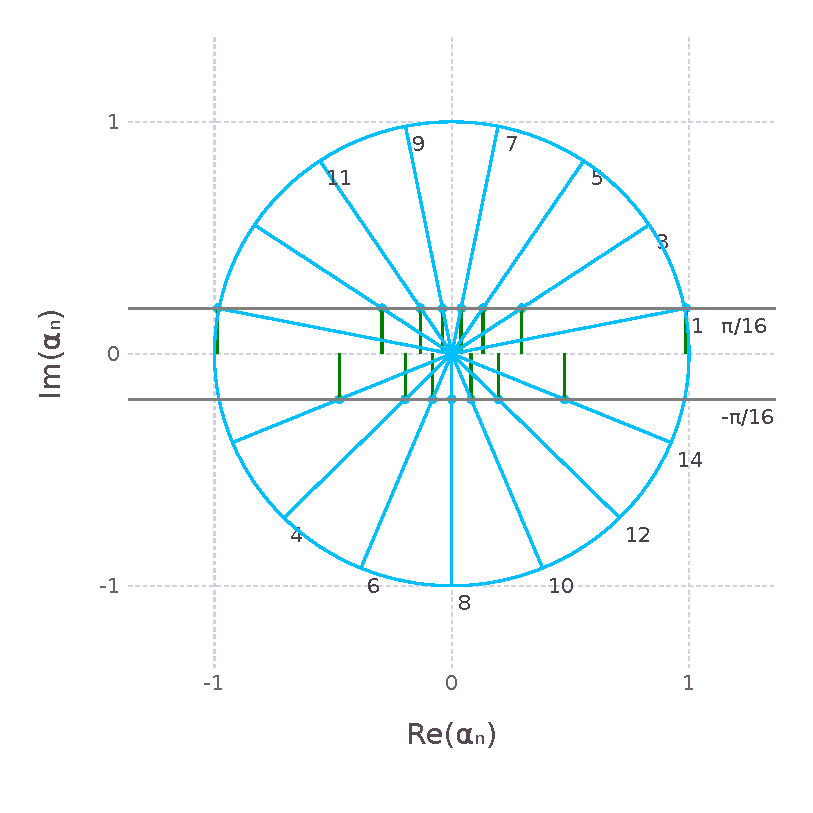
\includegraphics[natwidth=13cm,natheight=13cm]{pythagorean-16.pdf}
	\caption[Pythagorean coefficients for $p=16$]{Complex plane geometry of the Pythagorean coefficients $\alpha_n$ of period $p=16$. Blue points represent the location of the coefficients in the complex plane. Green lines illustrate the projection of the real component. Grey lines illustrate the imaginary component $\pm \frac{\pi}{16}$.}
	\label{fig:pythagorean-16}
\end{figure}
\begin{figure}[!ht]
	\centering
	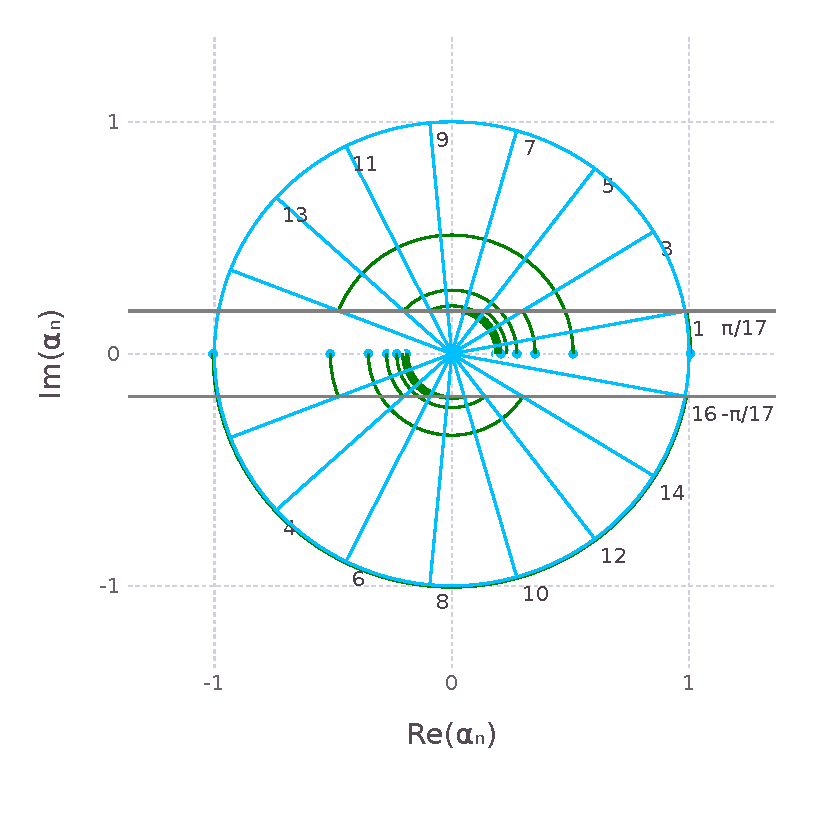
\includegraphics[natwidth=13cm,natheight=13cm]{pythagorean-17.pdf}
	\caption[Pythagorean coefficients for $p=17$]{Complex plane geometry of the Pythagorean coefficients $\alpha_n$ of period $p=17$. Blue points represent the location of the coefficients in the complex plane. Green lines carry the amplitude though to the intersection of the phase with the imaginary component $\pm \frac{\pi}{17}$.}
	\label{fig:pythagorean-17}
\end{figure}